As previously mentioned, there are two main issues that are being addressed for
forensics of \gls{SNF}: database issues and speed of characterization. Many
have begun considering computational approaches to nuclear forensics problems,
such as the INDEPTH tool for inverse depletion and decay analysis
\cite{weber_2006, weber_2010, weber_2011}. This tool uses an iterative
optimization method involving many forward simulations to obtain reactor
parameters of interest given some initial values. 

Another approach utilizes artificial intelligence to solve nuclear forensics
problems, such as implementing searching algorithms for the database comparison
step \cite{gey_search} and machine learning for determining reactor parameters
from \gls{SNF} characteristics \cite{dayman_feasibility_2013, nicolaou_2006,
nicolaou_2009, nicolaou_2014, robel_2009, jones_viz_2014, jones_snf_2014}.  A
variety of statistical and machine learning tools have been used to
characterize spent fuel by predicting categories or labels (e.g., reactor type, fuel
type) as well as predicting values (e.g., burnup, initial enrichment, cooling
time). The former uses classification algorithms and the latter uses regression
algorithms, many of which can be altered to perform both classification and 
regression.

As shown in Figure \ref{fig:supervised}, a typical (supervised) machine
learning workflow begins with a training data set, which has a number of
instances.  Each instance has some attributes (aka features) and a label, which
can be a categorical label or discrete/continuous values.  The training data
are then inserted into a statistical learner; this calculates some objective,
minimizes or maximizes that objective, and provides some model. This model is
typically evaluated using a test set that has the same set of attributes and
labels (but different instances). The comparison of what the model predicts and
the actual label gives the \textit{testing error}. Depending on the performance
and application, the model may need improvement from more training and/or some
changes in the algorithm parameters. Once the model is performing well enough,
it is finalized; then a user can provide a single instance and a value can be
predicted from that. 

\begin{figure}[h!]
  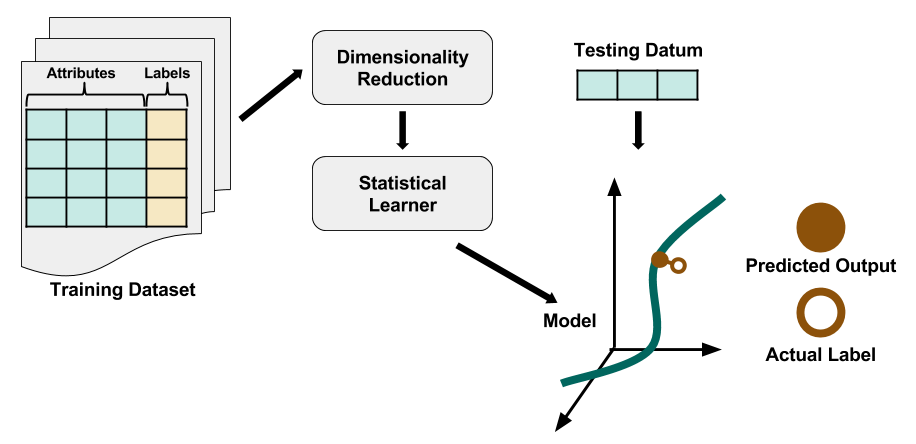
\includegraphics[width=\linewidth]{./chapters/intro/SupervisedRegression.png}
  \caption{Schematic represnting the typical workflow of a statistical learning regression algorithm.}
  \label{fig:supervised}
\end{figure}

This work evaluates to what degree statistical methods will be able to predict
reactor parameters with respect to the type of training data used.  There is
some promising work discussed in Section \ref{sec:stats4nf} that shows certain
applications of machine learning can provide an additional tool for solving the
forensics problem, both qualitatively (for visualization) and quantitatively
(for prediction).
